\documentclass[a4paper, oneside]{discothesis}

% use utf8 instead of latin1 when using LaTeX in windows
\usepackage[latin1]{inputenc}
\usepackage{listings}

\lstset{ %
	language=C++,
	keepspaces=true, 
	numbers=left, 
	basicstyle=\footnotesize, 
	numberstyle=\footnotesize, 
	tabsize=2,
	frame=single
	} 


%%%%%%%%%%%%%%%%%%%%%%%%%%%%%%%%%%%%%%%%%%%%%%%%%%%%%%%%%%%%%%%%%%%%%%%%%%%%%%%%%%%%%%%%%%%%%%%%%
% DOCUMENT METADATA

\thesistype{Bachelor Thesis}
\title{3D Depth Sensor on Mobile Devices (Acquisition, Calibration and 3D Reconstruction)}

\author{Lukas Bischofberger}
\email{lukasbi@ethz.ch}
\institute{Computer Vision and Geometry Group \\[2pt]
Institute for Visual Computing \\[2pt]
ETH Z�rich}

% You can put in your own logo here "\includegraphics{...}" or just comment the command
%\logo{}
%
\includegraphics{figures/cvg.png}

\supervisors{Dr. Amael Delaunoy\\[2pt] Prof.\ Dr.\ Marc Pollefeys}

% You can comment the following two commands if you don't need them
% \keywords{Keywords go here.}
% \categories{ACM categories go here.}

\date{\today}

%%%%%%%%%%%%%%%%%%%%%%%%%%%%%%%%%%%%%%%%%%%%%%%%%%%%%%%%%%%%%%%%%%%%%%%%%%%%%%%%%%%%%%%%%%%%%%%%%

\begin{document}

\frontmatter % do not remove this line
\maketitle

\cleardoublepage

\begin{acknowledgements}
	I would like to thank my supervisor Amael Delaunoy for his support and great help I received during the weekly meetings. Also I want to thank Professor Marc Pollefeys for offering me the opportunity to write my bachelor thesis at the Computer Vision and Geometry Group.
\end{acknowledgements}


\begin{abstract}
	The introduction of Kinect has made depth sensors available to the consumer world. This made it possible for basically everyone to have a 3D scanner at home. Systems like Kinect Fusion would give the possibility to easily get a 3D reconstruction of everything in front of the lens. 
	\newline
	The structure sensor by Occipital is the first mobile depth sensor and thus brings the possibility to have a mobile 3D scanner. We want to show that mobile depth data acquisition is possible and easy and also that this data performs well in 3D reconstruction applications.
\end{abstract}

\tableofcontents

\mainmatter % do not remove this line

% Start writing here

\chapter{Introduction}
	We want to use a state of the art mobile device and use it for depth data acquisition. For this we take advantage of the first mobile depth sensor, the structure sensor by Occipital. Further we will combine the depth data with the color images of the device for texturing the 3D model.
	\newline
	We want to show that this data then can be used to easily create a high quality 3D reconstruction. For this step we will use todays camera tracking and pose estimation algorithms like semi-direct monocular visual odometry or dense visual odometry.
	
	\section{Motivation}
		We want to show that with a mobile device like a smartphone or a tablet which today are omnipresent and a fairly low cost sensor we can perform high quality 3D scanning. This scans could be used in numerous applications in a daily life. Scans of rooms can for example be used to measure their dimensions and check for furniture to fit in. On the other hand such a scan could also be used for real estate advertisements. A last intention is also to show that 3D reconstruction with depth data performs better and faster than such with color images only.
	
	\section{Contribution}
		The contributions of our work are the following:
		
			\begin{itemize}
				\item An iOS application for the depth and color data acquisition which is based on the Structure SDK. It allows viewing and recording of RGBD data as well as camera calibration.
				\item An offline pipeline for the recorded data to perform estimation of the camera motion and 3D reconstruction.
			\end{itemize}
	
	\section{Related work}
		The following work has already been done in either mobile 3D reconstruction without the use of depth sensors or in 3D reconstruction with depth data in general.
		
		\subsection{Kinect Fusion}
			Kinect Fusion\footnote{https://msdn.microsoft.com/en-us/library/dn188670.aspx} is an application which provides 3D scanning and model creation based on the Kinect sensor. The user can paint a scene with the Kinect camera and simultaneously see, and interact with, a detailed 3D model of the scene. Kinect Fusion runs on a Desktop PC with the sensor attached by wire. The reconstruction and estimation of the camera movement is based on the tracking of the camera through the depth map. Further there exist possibilities to color the constructed models or to apply shading.
			
		\subsection{Live Metric 3D reconstruction on Mobile Phones}
			This paper \cite{paper1} proposes a complete on-device approach for 3D reconstruction. It uses a monocular hand-held device without any depth sensor. The reconstruction process is solely based on color images but the camera motion estimation takes advantage of the device own inertial sensors. Furthermore the paper proposes an efficient and accurate multi-resolution scheme for dense stereo matching which takes into account the restricted computational capabilities of the mobile device.
			
		\subsection{3D scanner}
			In the industry products like NextEngine 3 Scanner\footnote{http://www.nextengine.com/} have been available for some time. This scanner has a laser for high precision scanning and thus obtains far higher quality models than the approaches described before. It also features export to industry standard applications and allows easy printing of the scans. On the other side you need special equipment which is considerably more expensive than consumer electronic devices.

\chapter{Data acquisition}

	In this chapter we give a detailed description on how the data acquisition on mobile devices is performed. In a first step we describe the use of the structure sensor, it's mechanism and how we obtain the data in a meaningful way. Then we describe the relation between the depth data and color images taken from the device camera. In a third step we will show how to perform camera calibration and combine all the data to RGBD images. 

	\section{Mobile depth acquisition}
		The structure sensor is a so called structured-light 3D scanner. It possesses an infrared structured light projector and a corresponding camera system\footnotemark[1]. The projector projects a infrared mesh onto the scene which the camera records from a slightly different angle. The three-dimensionally shaped surface produces a distorted mesh relative to the viewing camera which is then able to perform a geometric reconstruction of the surface shape.
		
		\begin{figure}[h]
			\centering
			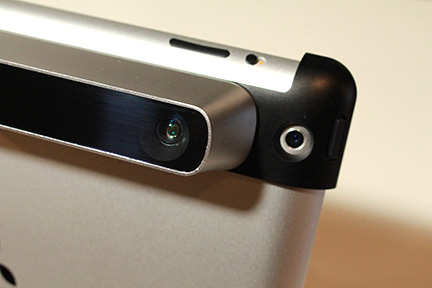
\includegraphics[width=\textwidth/3]{figures/ipad-sensor}
			\footnote{http://structure.io/static/occipital/images/v1/getstarted/ipad\_camera\_centered.jpg}
			\caption{Structure sensor on iPad}
			\label{fig:sensor}
		\end{figure}

		The sensor is connected to the device by cable, in our case to the iPad through the lightning port. We use the Structure SDK\footnotemark[1] as an interface between our application and the sensor hardware. This provides us with an infrared / color image pair for camera calibration and a depth map / color image pair for the data acquisition process. 
		
		Originally we wanted to perform the mobile data acquisition on an Android device because the structure sensor as well as Android support OpenNI. Including the OpenNI libraries, drivers and the OpenCV libraries in the Android NDK turned out to be far harder than expected. Even though the iOS platform is more restricted and it's harder to extract data from the mobile device, it was easier to go with that platform.
		
		\begin{figure}[h]
			\centering
			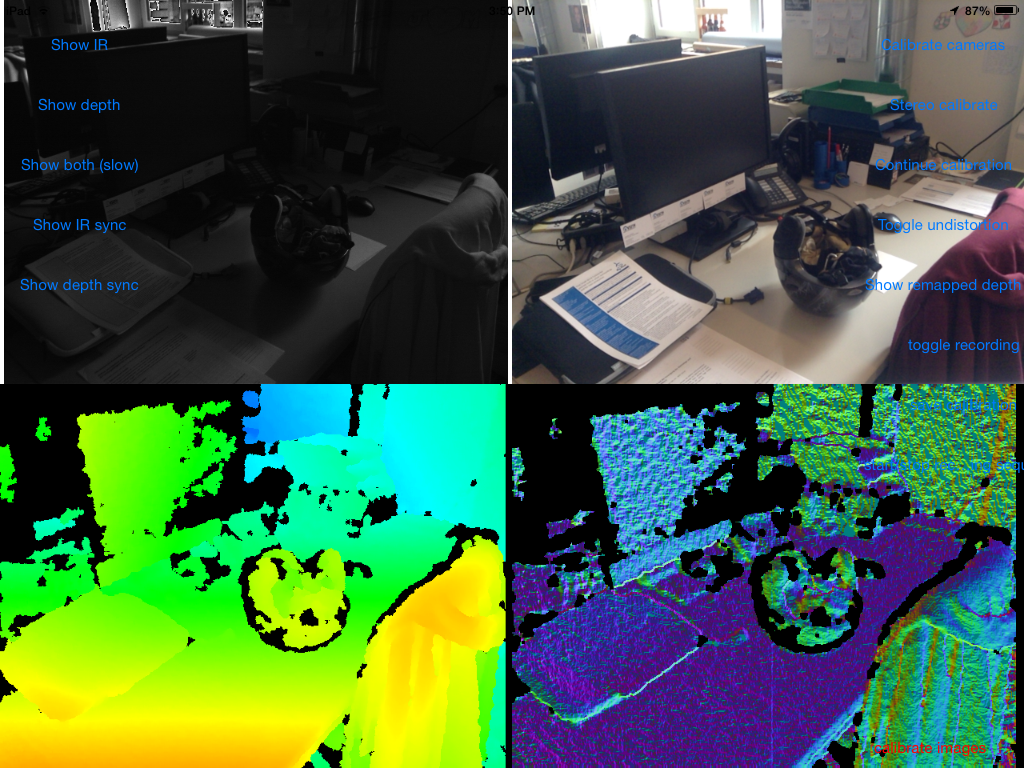
\includegraphics[width=\textwidth/2]{figures/acquisition}
			\caption{Data acquisition screen}
			\label{fig:acquisition}
		\end{figure}
		
		\footnotetext[1]{http://structure.io/developers}
		

	\section{RGB and Depth Camera Calibration}

		For the camera calibration we make use of the pinhole model. Hence we want to calibrate the sensor's depth camera and the device's RGB camera for their intrinsics. As a result we will find the camera matrices and lens distortion coefficients for both cameras. After having obtained a satisfying calibration for both cameras we can use the computed intrinsics to perform a stereo camera calibration, thus finding the camera extrinsic parameters. 
		
		\subsection[Pinhole camera model]{Pinhole camera model\footnote{http://docs.opencv.org/modules/calib3d/doc/camera\_calibration\_and\_3d\_reconstruction.html}}
		
			\begin{equation}
				s p = K(RP + t)
			\end{equation}
			
			where $P = \begin{pmatrix}X\\Y\\Z\end{pmatrix}$ is a 3D point in the world coordinate space and $p = \begin{pmatrix}u\\v\\1\end{pmatrix}$ is the projection of $P$ in the camera frame in pixels.
			
			\begin{equation}
				K =
				\begin{bmatrix}
					f_x & 0 & c_x\\
					0 & f_y & c_y\\
					0 & 0 & 1
				\end{bmatrix}
			\end{equation}
						
			$K$ is called the camera matrix or a matrix of intrinsic parameters, $f_x, f_y$ are the focal lengths expressed in pixel units and $(c_x,c_y)$ is the principal point that is usually located at the image center. Furthermore we have the rotation matrix $R$ and the translation vector $t$. We will refer to $[R|t]$ as the matrix of extrinsic parameters. It is used to describe the camera motion around a static scene in our case. In a more general application it would also describe the rigid motion of an object in front of the camera.  
						
			\begin{equation}
				R =
				\begin{bmatrix}
					r_{11} & r_{12} & r_{13}\\
					r_{21} & r_{22} & r_{23}\\
					r_{31} & r_{32} & r_{33}
				\end{bmatrix},
				t=
				\begin{bmatrix}
					t_1\\
					t_2\\
					t_3
				\end{bmatrix}
			\end{equation}
			
			\begin{figure}[h]
				\centering
				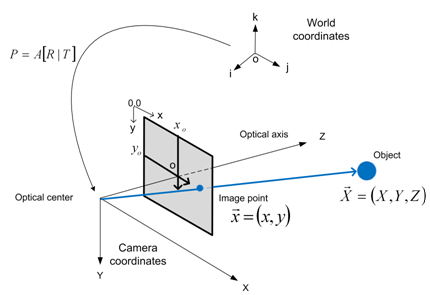
\includegraphics[width=0.6\textwidth]{figures/pinhole}
				\footnote{http://archimede.bibl.ulaval.ca/archimede/fichiers/25229/25229\_35.png}
				\caption{Pinhole camera model}
				\label{fig:pinhole}
			\end{figure}
			
			Because real lenses usually have some radial and tangential distortion $k_1$ to $k_6$ and $p_1$ and $p_2$ are introduced and the camera model is extended as follows.
			
			\begin{equation}
				\begin{pmatrix}x\\y\\z\end{pmatrix} = R \begin{pmatrix}X\\Y\\Z\end{pmatrix} + t
			\end{equation}
			\begin{equation}
				x' = \frac{x}{z}, y' = \frac{y}{z}
			\end{equation}
			\begin{equation}
				\begin{split}
					x'' = x'\frac{1 + k_1 r^2 + k_2 r^4 + k_3 r^6}{1 + k_4 r^2 + k_5 r^4 + k_6 r^6} + 2 p_1 x' y' + p_2(r^2 + 2 x'^2)  \\ 
					y'' = y'\frac{1 + k_1 r^2 + k_2 r^4 + k_3 r^6}{1 + k_4 r^2 + k_5 r^4 + k_6 r^6} + p_1 (r^2 + 2 y'^2) + 2 p_2 x' y'  \\
					\text{where} \quad r^2 = x'^2 + y'^2  \\
				\end{split}
			\end{equation}
			\begin{equation}
				\begin{split}
						u = f_x*x'' + c_x \\ v = f_y*y'' + c_y
				\end{split}
			\end{equation}
		
		\subsection{Single Camera Calibration}
			We perform calibration on a chessboard pattern, say we're looking for a certain amount of corners in a picture. Those corners must be arranged in a certain grid with specific width and height. Furthermore we specify the real distance between two corners in millimeters. When looking at a series of images which all contain the same pattern from different viewpoints we can estimate the  distortion coefficients of the lens and the camera matrix.
			
			We can now use the calibrations of both cameras and display an undistorted color image and an undistorted depth map. But we can also use the results of this step for the upcoming stereo calibration as input parameters. We can control the quality of the calibration by looking at the RMS of the back-projection error. It usually should lie between 0.1 and 1.0 pixels. For the color image we usually get something around 0.2 which is quite good and for the infrared image an error of around ??.
			
			\begin{figure}[h]
				\centering
				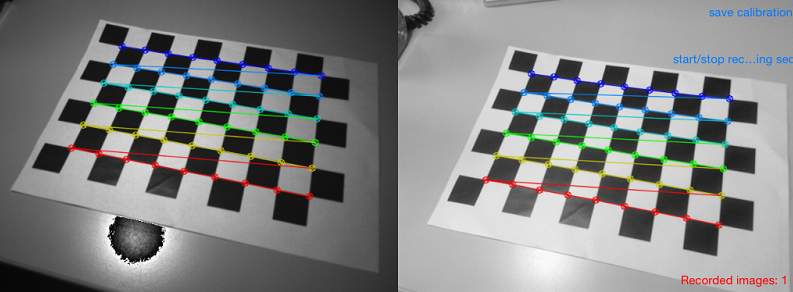
\includegraphics[width=0.8\textwidth]{figures/calib1}
				\caption{IR and RGB images with the calibration pattern}
				\label{fig:calib}
			\end{figure}
			
			\begin{figure}[h]
				\centering
				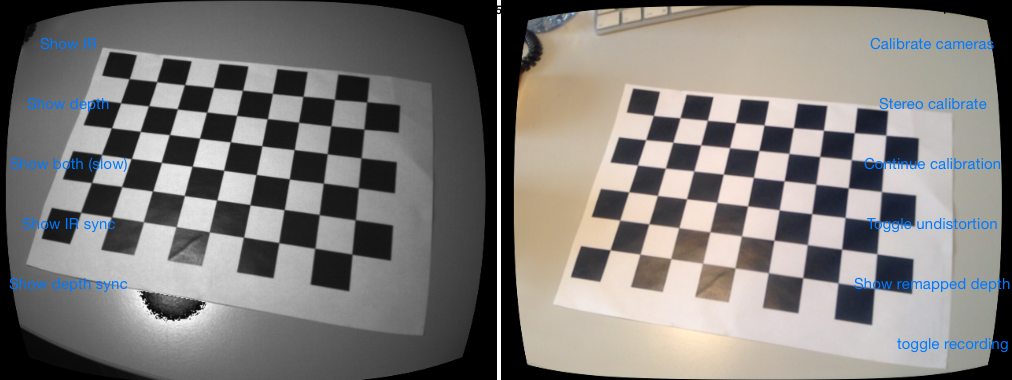
\includegraphics[width=0.8\textwidth]{figures/undist}
				\caption{Undistorted IR and RGB images}
				\label{fig:undist}
			\end{figure}
		
		\subsection{Stereo Calibration}
			In the stereo calibration we try to estimate the extrinsic parameters. So we want to find the rotation and translation between the two camera centers. We will use the precomputed camera matrices and intrinsic parameters from the previous section as well as synchronized infrared / color image pairs as input.
			
			The algorithm estimates the 
			$\begin{pmatrix}
			X \\ Y \\ Z
			\end{pmatrix}$
			coordinates for all points of the calibration pattern in the world coordinate system based on a series of images from a certain camera. On the other hand it also creates stereo pairs of infrared and color images, thus taking images form different cameras and so estimates the relative transformation between the two cameras. Therefore we will retrieve the rotation matrix $R$ and the translation vector $t$ which describe the dislocation of the infrared sensor from the color camera or vice versa.
			
			\begin{figure}[h]
				\centering
				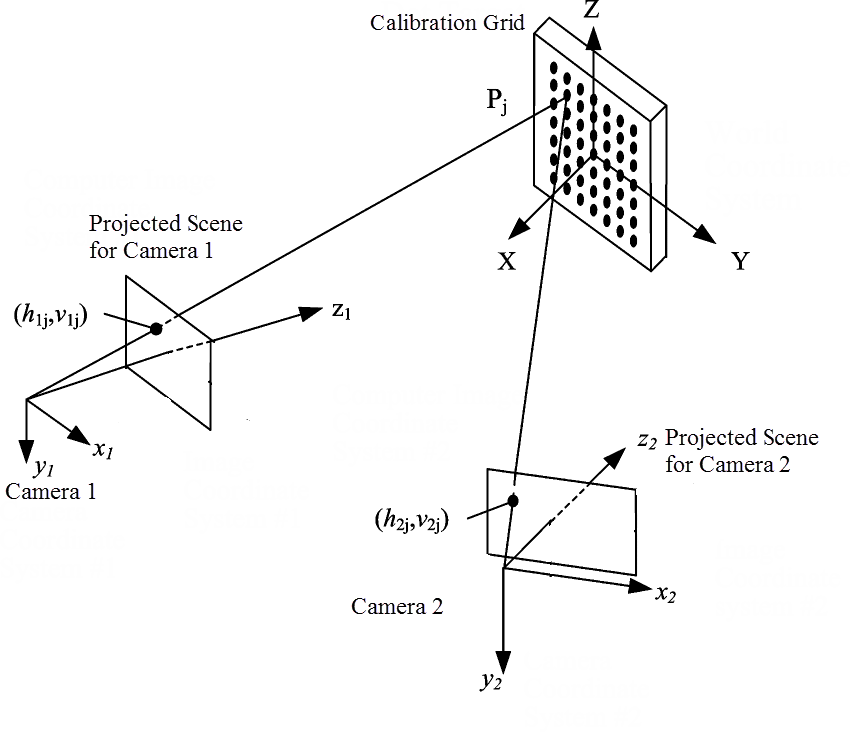
\includegraphics[width=0.8\textwidth]{figures/stereo}
				\caption{Stereo camera calibration}
				\label{fig:stereo}
			\end{figure}
			
			For better understanding we can also represent $R$ and $t$ as a combination of two camera to world  transformations.
			
			\begin{equation}
				R = R_{rgb}(R_{ir})^{T}
			\end{equation}
			
			\begin{equation}
			T = T_{rgb} + RT_{ir}
			\end{equation}
			
			Where $R_{rgb}$ and $t_{rgb}$ are the extrinsic parameters of the color camera and vice versa for the infrared camera. Thus $R$ and $t$ define the transformation from the infrared coordinate system to the color camera coordinate system.
			
			We can also control the quality of the stereo calibration by looking at the RMS like with the single camera calibration. Here the error is usually a little higher but values between 0.5 and 1.5 yielded good results.
						
%			\begin{equation} \label{eq:prgb}
%				P_{rgb} = R_{rgb} * p_{rgb} + t_{rgb}
%			\end{equation}
%			
%			\begin{equation} \label{eq:pir}
%				p_{ir} = R_{ir} * P_{ir} + t_{ir}
%			\end{equation}
%			
%%			Combining \ref{eq:prgb} and \ref{eq:pir} will leave us with
%			Hence we get the rotation matrix and the translation vector between the two camera centers. 
%			
%			\begin{equation}
%				R = R_{ir}(R_{rgb})^{T}, t = t_{ir} + Rt_{rgb}
%			\end{equation}			
%			
%			\begin{equation}
%				p_{rbg} = K_{rgb} * R * K_{ir}^{-1} * p_{ir} + t 
%			\end{equation}

	\TODO{side by side of rectified image pair?}
		
	\section{Depth re-projection}
		As we now have obtained the camera specific parameters and also the extrinsic parameters the only thing left is to combine this information. Thus we want to create an RGBD image with depth and color information. For storage reasons we will not create a four channel image but use a three channel RGB and a single channel depth image.
		
		Thus for the first time now we record a depth image with the sensor staying at the same spot relative to the color camera as for the calibration. Hence we have a depth map / color image pair which we combine using the pinhole camera model and all the parameters we obtained throughout calibration.  We will do the following procedure for every pixel in the depth image. First we project it into its cameras coordinate system using the camera matrix. Then we apply the rotation and translation obtained during stereo calibration to transform the point into the color camera coordinate system. And last we back-project the point into the color camera frame to obtain its pixel coordinates, whereas the $z$ coordinate of the point in the color camera coordinate system represents its depth.   
		
		Mathematically this operation is formulated the following way whereas we use these variables:\\
		$p_{ir}:$ Point in the infrared camera frame\\
		$P_{ir}$: 3D point in the infrared camera's coordinate system\\
		$P_{rgb}$: 3D point in the color camera's coordinate system\\
		$p_{rgb}$: Projection of $P_{rgb}$ onto the color camera frame\\
		
		\begin{equation}
			P_{ir} = inv(K_{ir})*p_{ir}
		\end{equation}
		
		\begin{equation}
			\label{eq:Prgb}
			P_{rgb} = R * P_{ir} + t
		\end{equation}
		
		\begin{equation}
			p_{rgb} = K_{rgb} * P_{rgb}
		\end{equation}
		
		\begin{equation}
			depth of p_{rgb} = P_{rgb}.z
		\end{equation}
		
		\begin{figure}[h]
			\centering
			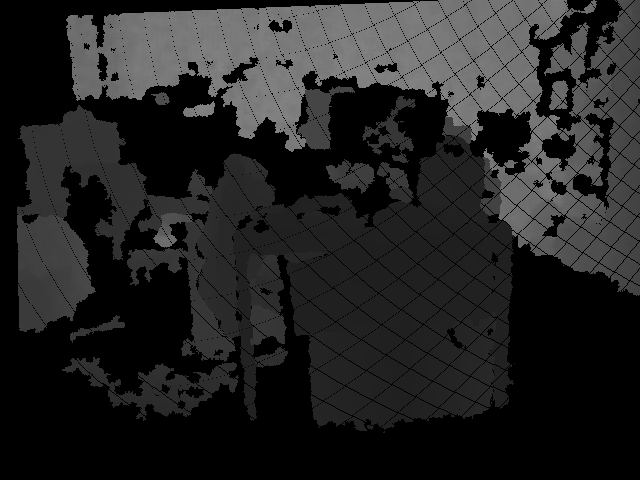
\includegraphics[width=0.8\textwidth]{figures/reprojection}
			\caption{Re-projected depth image}
			\label{fig:reprojection}
		\end{figure}
		
		Because we project the depth values in the color frame we always lose some information. E.g. those values which would be projected outside the color frame can't be used anymore. We also see some aliasing effects throughout the entire image. This could be solved by a triangulation approach.
		
		\TODO{show depth and depth re-projected next to each other}

		\TODO{Show RGBD.}
	
\chapter{3D reconstruction}
	To obtain a 3D reconstruction we will rely on the fastfusion pipeline \cite{fastfusion}. It takes as input color image / depth map pairs and their corresponding camera poses. For that reason we use the semi-direct visual odometry pipeline to track the camera center based on the color image sequence and estimate the camera trajectory.

	\section{Camera tracking - SVO}
		SVO: Semi-Direct Monocular Visual Odometry is an algorithm that performs motion estimation without relying on  costly feature extraction and robust matching \cite{svo}. Instead it operates on pixel intensities which results in subpixel precision at high frame rates. In general we leave the procedure of the SVO pipeline unchanged. We just extended the code to also export the 
		$\begin{pmatrix}
			u \\ v
		\end{pmatrix}$
		coordinates and the corresponding $Z$ values of the tracked features. Besides that we obtain the world to camera translation and rotation matrices as a result from the algorithm. 
		
		\TODO{	How was the performance of SVO on the dataset?
			-> iPad not fast enough, thus too large gaps between images -> bad tracking}
		
	\section{Camera tracking - bundler / visualsfm}
		Operates with sift, no consecutive frames, matches all images. Takes longer, but also bad performance
	
	\section{Scale estimation}
		Because SVO operates in its own coordinate system, which is based on the features it is tracking, the $Z$ values which is the estimated depth of the features don't align with the real depth.
		
		That means that for a feature at position 
		$\begin{pmatrix}
		X \\ Y \\ Z
		\end{pmatrix}$
		which is projected to 
		$\begin{pmatrix}
		u_i \\ v_i \\ z_i
		\end{pmatrix}$
		in the camera frame $z_i$ usually doesn't equal the $z$ value of $P_{rgb}$ in \ref{eq:Prgb}, here denoted as $d_i$. Therefore we need to introduce a scale factor which corrects the depth difference. We used a simple least squares approach:
		
		\begin{equation}
			\sum_{i=0}^{width * height * images} (d_i - s*z_i)* z_i = 0
		\end{equation} 
		
		Subsequently we will scale every camera pose by this factor $s$. Because the camera pose is computed by
		\begin{equation}
			\label{eq:camera_center}
			c_j = -R_j^T*t_j
		\end{equation}
		
		where $c_j$ is the camera center of the $j$'th camera and $[R_j|t_j]$ is the camera to world coordinate system transformation matrix. Therefore it is enough to scale the vector $t_j$ by a factor of $s$ to account for the false depth.
		
	\section{Pointcloud}
		To obtain a visual conformation that the scale estimation succeeded we converted the depth map / color image pairs to pointclouds. For this we computed the camera pose as in \ref{eq:camera_center}, to get a visual of the image origin. Then we used the extrinsic parameters of the color camera to transform the RGBD image to a pointcloud. 
		
		\begin{equation}
			P_i = R_{rgb}^{T}(K_{rgb}^{-1}p_i - t_{rgb})
		\end{equation}where $p_i$ is the vector 
		$\begin{pmatrix}
			u_{i}d_{i} \\ v_{i}d_{i} \\ d_{i}
		\end{pmatrix}$, $u$ and $v$ being the pixel coordinates of the depth $d$ in the color camera frame. Accordingly the color of $p_i$ is the RGB value at $(u_i,v_i)$.
		
		\TODO{put pointcloud img}
	
	\section{Dense reconstruction}
		To perform the dense 3D reconstruction we use the fastfusion pipeline \cite{fastfusion}. 
		\TODO{some more information on fastfusion}
	
		\begin{figure}[h]
			\centering
			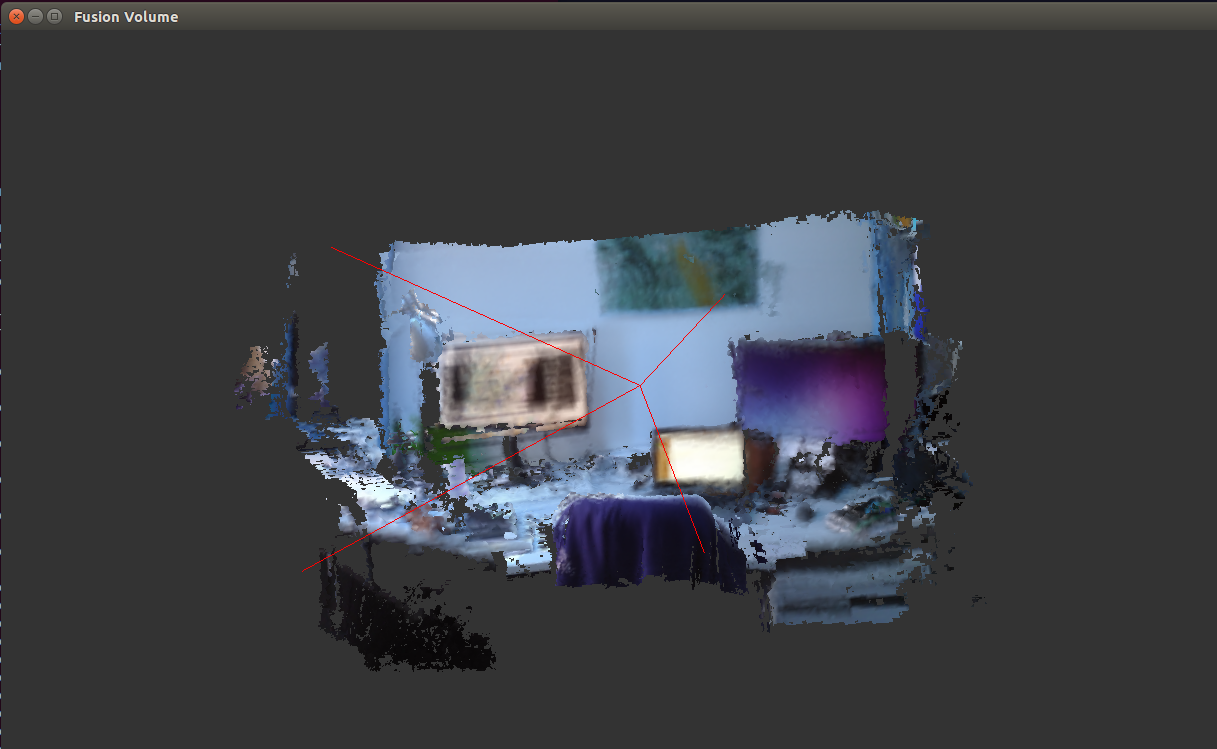
\includegraphics[width=\textwidth]{figures/reconstruction}
			\caption{Re-projected depth image}
			\label{fig:reprojection}
		\end{figure}
		
	\section{App integration}
		
%		\begin{figure}[h]
%			\centering
%			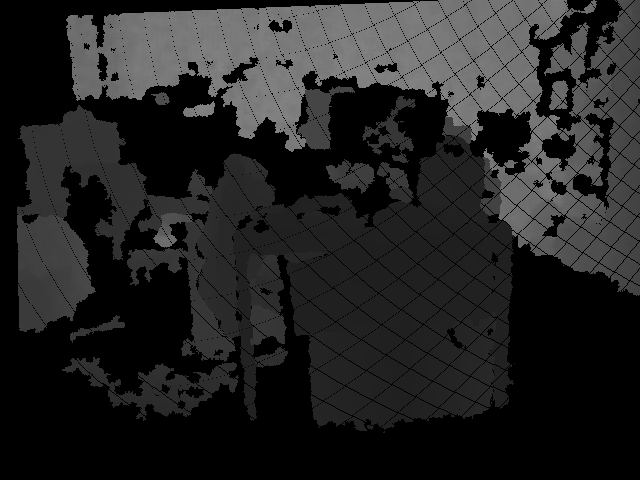
\includegraphics[width=0.8\textwidth]{figures/reprojection}
%			\caption{Re-projected depth image}
%			\label{fig:reprojection}
%		\end{figure}
			
			
\chapter{Conclusion}

	

\chapter{Future work}

%And here we cite an external document~\cite{TestReference}.

% This displays the bibliography for all cited external documents. All references have to be defined in the file references.bib and can then be cited from within this document.
\bibliographystyle{splncs}
\bibliography{references}

% This creates an appendix chapter, comment if not needed.
\appendix
\chapter{Code}

	\section{Depth reprojection}
		\begin{lstlisting}
for (int row = 0; row < depthRaw.rows; ++row) {
	for (int col = 0; col < depthRaw.cols; ++col) { 
	
		// not mapped depth image
		ptrDepth[depthRaw.cols * row + col] = 
		(uint16_t)ptrOrig[depthRaw.cols * row + col];
		
		// get depth for remapping
		double depthVal = (double)ptrOrig[depthRaw.cols*row + col];
		
		// Map depthcam depth to 3D point
		Mat_<double> P3D = Mat_<double>(3,1);
		
		P3D(0) = (col - camera1.at<double>(0,2)) 
		* depthVal / camera1.at<double>(0,0);
		P3D(1) = (row - camera1.at<double>(1,2)) 
		* depthVal / camera1.at<double>(1,1);
		P3D(2) = depthVal;
		
		// Rotate and translate 3D point
		Mat_<double> P3Dp;
		P3Dp = (R*P3D) + T;
		
		// Project 3D point to rgbcam
		double xrgb = (P3Dp(0) * camera2.at<double>(0,0) / P3Dp(2)) 
		+ camera2.at<double>(0,2);
		double yrgb = (P3Dp(1) * camera2.at<double>(1,1) / P3Dp(2)) 
		+ camera2.at<double>(1,2);
		double nDepth = P3Dp(2);  
		
		// "Interpolate" pixel coordinates (Nearest Neighbors)
		int px_rgbcam = cvRound(xrgb);
		int py_rgbcam = cvRound(yrgb);
		
		// Handle 3D occlusions
		uint16_t &depth_rgbcam = 
		ptrMapped[depthRaw.cols * py_rgbcam + px_rgbcam];
		uint16_t &depth_rgbcamScale = 
		ptrMappedScale[depthRaw.cols * py_rgbcam + px_rgbcam];
		
		if(px_rgbcam - depthRaw.cols < 0 
		&& py_rgbcam - depthRaw.rows < 0) {
			if(depth_rgbcam == 0 || (uint16_t)nDepth < depth_rgbcam) {
				depth_rgbcam = 5*(uint16_t)nDepth;
			}
		}   
	}
}
		\end{lstlisting}

\end{document}